%\documentclass[doc,11pt]{apa6}
\documentclass[man,11pt]{apa6}
%\documentclass[jou,11pt]{apa6}
\usepackage{apacite}
\usepackage{setspace}
\usepackage{subfigure}
\usepackage{url}
\newcommand{\bibnodot}[1]{}

% margins
\setlength{\textheight}{9true in}
\setlength{\textwidth}{6.25true in}
\setlength{\topmargin}{-.43true in}
\setlength{\headheight}{.17true in}
\setlength{\headsep}{.25true in}
\setlength{\footskip}{.42true in}
\setlength{\topskip}{12pt}
\setlength{\oddsidemargin}{0.1true in}

\title{Predicting Weeding Decisions: Results}
\shorttitle{Predicting Weeding Decisions: Results}

\author{Kiri L. Wagstaff}
\affiliation{San Jose State University}
\note{\today}

\begin{document}
\maketitle

\section{Data Set Description}

This data set was obtained from Diane Klare and Lori Strethers of
Wesleyan University in March, 2015.
%
It contains 94,174 items identified as weeding candidates during a
large-scale weeding project that took place from 2011 to 2014 at
Wesleyan under the direction of Pat Tully.  Each item is marked to
indicate whether it was withdrawn or kept as a result of the weeding
project.

The goal of this project is to assess whether automated machine
learning classifiers can be trained to successfully reproduce human
judgments about whether items should be withdrawn or kept.

\section{Data Preprocessing}

I used the data set to create the following representation of items:
\singlespacing
\begin{center}
\begin{tabular}{|l|p{4.5in}|}
\hline
 {\em age} & Number of years between Publication Year and 2014, when the
  data was collected (integer ranging from 25 to 402). \\
 {\em checkouts} & The data set reports the number of checkouts
  since 1996.  The data set only includes items with fewer than 2
  checkouts, so this value is either 0 or 1 for all items. \\
 {\em shelftime} & Number of days since the last checkout, or -1
  if no last checkout is known (integer ranging from 763 to 6792, or -1). \\
 {\em uslib} & Number of U.S. libraries with a copy of this item,
  based on OCLC holdings records (integer ranging from 31 to 7634). \\
 {\em peerlib} & Number of peer libraries with a copy of this item,
  based on OCLC holdings records (integer ranging from 2 to 3;
  selection criteria for the data set included presence in at least
  two peer libraries). \\
 {\em hathicopy} & Does a copyrighted digital version exist in the
 Hathi Trust?  (boolean)\\
 {\em hathipub} & Does a public domain digital version exist in the
 Hathi Trust?  (boolean)\\
 {\em facultykeep} & Number of Wesleyan faculty votes to keep the item
  (integer ranging from 0 to 15). \\
 {\em librariankeep} & Number of Wesleyan librarian votes to keep the
  item (integer ranging from 0 to 1). \\
\hline
 {\em decision} & ``Withdraw'' or ``Keep''. \\
\hline
\end{tabular}
\end{center}
\doublespacing

I encountered some oddities in the data set.  In consultation with
Lori Strethers, I applied the following data cleaning steps:
\begin{itemize}
\item One item (``Germany's stepchildren,'' by Solomon Liptzin) had a
  ``Publication year'' of 5704.  The correct value is 1944.  I updated it
  in the database.

\item Lori indicated that items that are marked as part of an
  ``enumeration'' (series) were handled separately with different
  criteria, so I excluded them from the data set.  This affected 8,141
  items. 

\item Some items had a ``Date of last checkout'' after 1996, but the
   ``Checkouts since 1996'' field was 0.  Lori identified two causes:
(1) ``Multi-volume sets assign last circ date to all items in the set,
  but the number of checkouts is only incremented for the item checked out.''
(2)  ``Standalone items were checked out but not returned, and the 
  number of checkouts is incremented only when the item is returned.''
For both kinds of cases, I set the number of checkouts to 1.  This
affected 1,052 items.

\item Some items had no value for ``Date of last checkout'', but the
  ``Checkouts since 1996'' field was 1.  Lori explained: ``For these
  you can assume that it was checked out between 1996 and 2003.
  (System migration in 2003: items that were still charged out had
  their checkout date migrated, but items that had been returned just
  had a counter incremented to indicate how many times they had
  circulated.)''
%
Because we cannot be confident about the last checkout date for these
items, I decided to omit them from the data set. This affected 18,346
items. 

\end{itemize}

\section{Data Analysis}

\begin{figure}
\centering
\subfigure[{\em age}: Full data set]{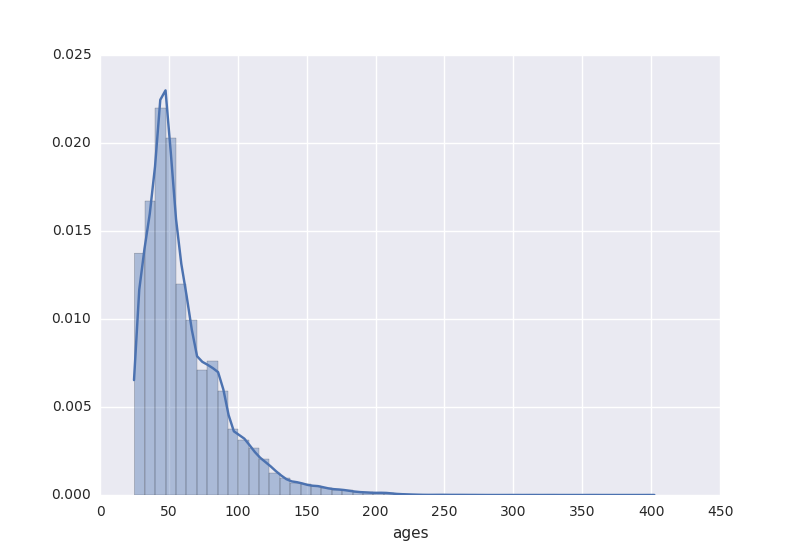
\includegraphics[width=3.1in]{../data/fig/hist-ages}} 
\subfigure[{\em age}: Split by decision]{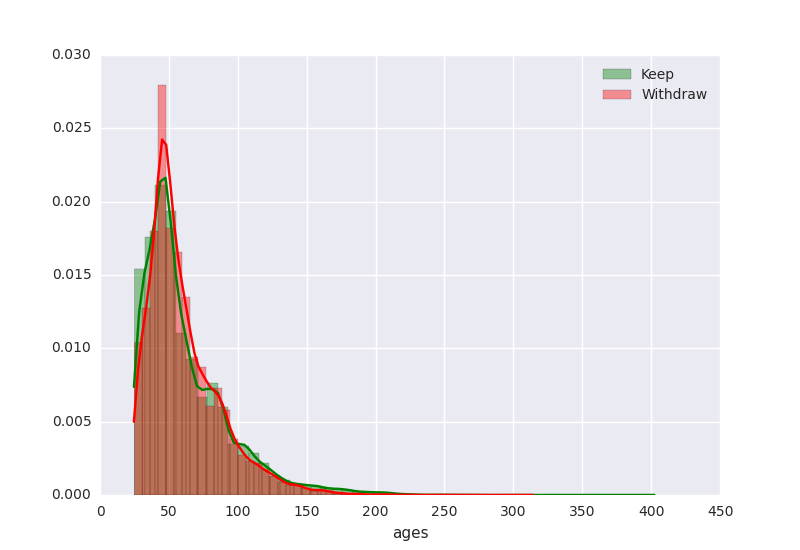
\includegraphics[width=3.1in]{../data/fig/hist-ages-split}}\\
\subfigure[{\em shelftime}: Full data set]{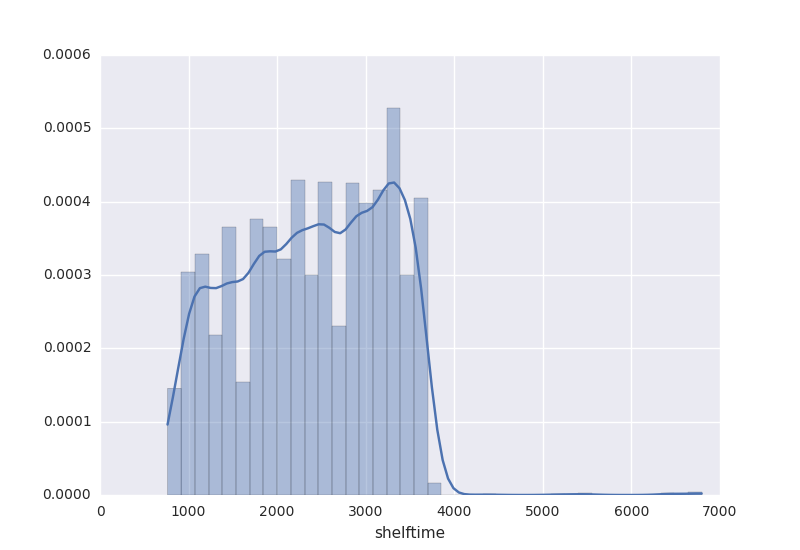
\includegraphics[width=3.1in]{../data/fig/hist-shelftime}} 
\subfigure[{\em shelftime}: Split by decision]{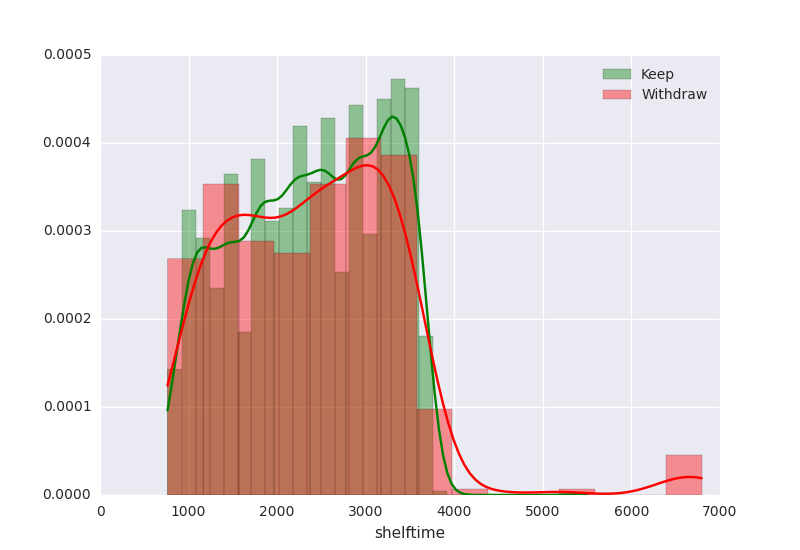
\includegraphics[width=3.1in]{../data/fig/hist-shelftime-split}}\\
\subfigure[{\em uslibs}: Full data set]{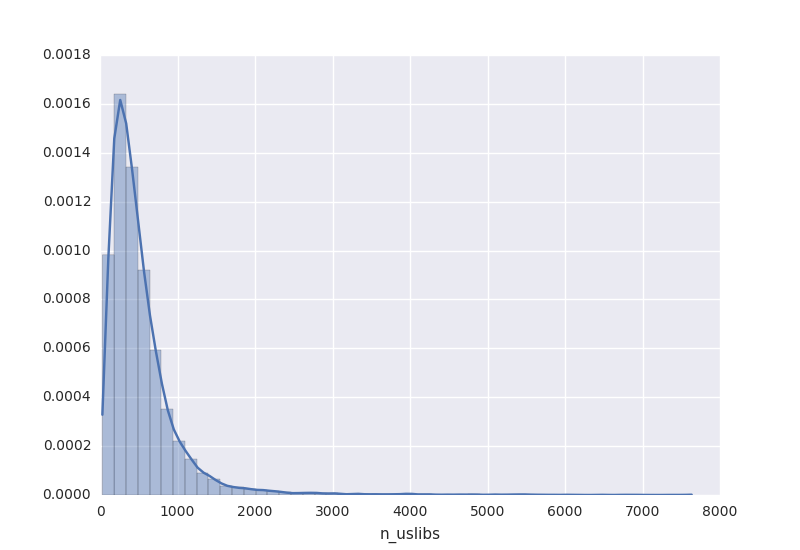
\includegraphics[width=3.1in]{../data/fig/hist-n_uslibs}}
\subfigure[{\em uslibs}: Split by
  decision]{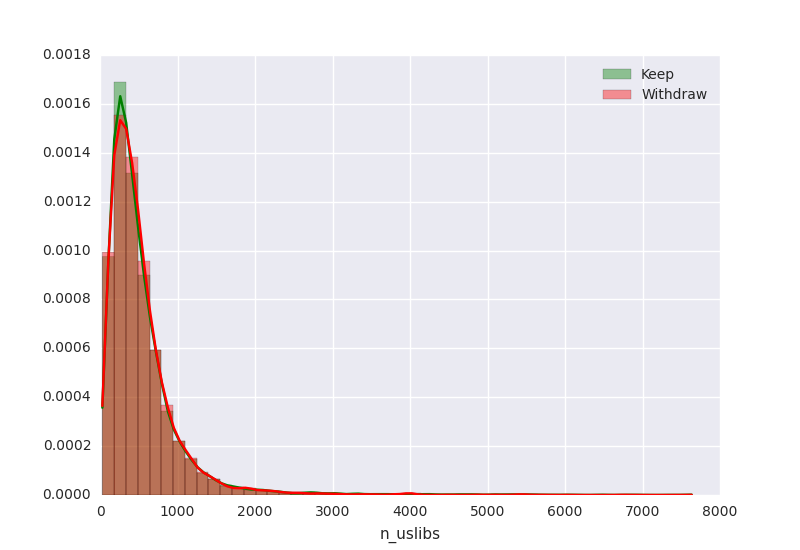
\includegraphics[width=3.1in]{../data/fig/hist-n_uslibs-split}}
\caption{Distribution of values observed for three variables (left
  column) as well as the distributions compiled separately for items
  marked ``Keep'' vs. ``Withdraw.''}
\label{fig:dist}
\end{figure}

The data set contains 67,687 items, 25,632 (38\%) of which are marked
``Withdraw'' and 42,055 (62\%) of which are marked ``Keep.''  

The minimum, mean, and maximum values for the four variables with more
than two distinct values are as follows:

\singlespacing
\begin{center}
\begin{tabular}{|l|ccc|}
\hline
Variable & Minimum & Mean & Maximum \\
\hline
 {\em age} & 25 & 61 & 402 \\
 {\em shelftime} & 763 & 2381 & 6792 \\
 {\em uslib} & 31 & 535 & 7634  \\
 {\em facultykeep} & 0 & 0 & 15 \\
\hline
\end{tabular}
\end{center}
\doublespacing

% Question: shelftime min is 763... was criteria that no checkout
% in last two years? I need to articulate their criteria above.

Figure~\ref{fig:dist} shows the distribution of values observed for
the first three variables (the fourth has very few non-zero values).
In general, we do not see a strong separation between ``Withdraw'' and
``Keep'' decisions for any single variable, except for {\em
  shelftime}, in which items with very large {\em shelftime} values
are more likely to be withdrawn, as we would expect.

For variables that take on only two possible values, I analyzed the
distribution of ``Keep'' adn ``Withdraw'' decisions.
%
The {\em checkouts} variable is dominated by items that have never
been checked out: 92\% of items in the data set have 0 checkouts.
The probability of an item being withdrawn, $P(W)$, given that it has
0 checkouts, is much higher than if it has 1 checkout (0.41 vs.~0.07).
The probability that an item is withdrawn, across the whole data set,
is 0.38. 

\singlespacing
\begin{center}
\begin{tabular}{|c|rr|rr|c|}
\hline
{\em checkouts} & Number & Fraction & Withdraw & Keep & $P(W)$\\ \hline
0 & 61,993 & 91.59\% & 25,252 & 36,741 & 0.41 \\
1 &  5,694 &  8.41\% &    380 &  5,314 & 0.07 \\
\hline
\end{tabular}
\end{center}
\doublespacing

The {\em peerlibs} variable is less strongly aligned with the weeding
decision, but there is still a difference between items that are held
by two peer libraries (60\% of the items, with $P(W) = 0.39$) versus
those held by three peer libraries (40\% of the items, with $P(W) =
0.36$).  The latter are less likely to be withdrawn.

\singlespacing
\begin{center}
\begin{tabular}{|c|rr|rr|c|}
\hline
{\em peerlibs} & Number & Fraction & Withdraw & Keep & $P(W)$\\ \hline
2 & 40,549 & 59.91\% & 15,991 & 24,558 & 0.39 \\
3 & 27,138 & 40.10\% &  9,641 & 17,497 & 0.36 \\
\hline
\end{tabular}
\end{center}
\doublespacing

Items in the Hathi Trust are more likely to be held in copyright
(56\%) than to be in the public domain (14\%).  For those items with a
copyrighted version in the Hathi Trust, the probability of being
withdrawn is higher (0.41) versus those items with a public domain
copy (0.37), which is very close to the data set average (0.38). 

\singlespacing
\begin{center}
\begin{tabular}{|c|rr|rr|c|}
\hline
{\em hathicopy} & Number & Fraction & Withdraw & Keep & $P(W)$\\ \hline
False & 29,518 & 43.61\% & 10,126 & 19,392 & 0.34 \\
True  & 38,169 & 56.39\% & 15,506 & 22,663 & 0.41 \\
\hline
\end{tabular}
\end{center}
\doublespacing

\singlespacing
\begin{center}
\begin{tabular}{|c|rr|rr|c|}
\hline
{\em hathipub} & Number & Fraction & Withdraw & Keep & $P(W)$\\ \hline
False & 58,149 & 85.91\% & 22,099 & 36,050 & 0.38 \\
True  &  9,538 & 14.10\% &  3,533 &  6,005 & 0.37 \\
\hline
\end{tabular}
\end{center}
\doublespacing

Finally, 13\% of the items have a value of 1 for the {\em
  librariankeep} variable.  There is a very strong relationship
between librarian votes and final decisions, as we expect: 98\% of
items with a ``Keep'' vote are kept (i.e.,~$P(W) = 0.02$).  The 211
items that were withdrawn despite a ``Keep'' vote were determined to
be either lost or duplicates of other items.

\singlespacing
\begin{center}
\begin{tabular}{|l|cc|cc|c|}
\hline
{\em librariankeep} & Number & Fraction & Withdraw & Keep & $P(W)$\\ \hline
0 & 58,754 & 86.80\% & 25,411 & 33,343 & 0.43 \\
1 &  8,933 & 13.20\% &    211 &  8,712 & 0.02 \\
\hline
\end{tabular}
\end{center}
\doublespacing


\section{Experimental Results}

I divided the data set randomly into two parts, one for training and
one for testing.  I evaluated several machine learning algorithms on
both data sets, after training.  I also evaluated baseline approaches
that predict ``Withdraw'' or ``Keep'' for all items.

To evaluate the agreement between the machine predictions and the
human decisions, I calculated the accuracy (fraction of predictions
that match human decisions) and the $\phi$ statistic (a measure of
agreement).  I also report the $p$-value at which the $\phi$ agreement
is considered to be statistically significant.

Given this definition of a contingency table:

\singlespacing
\begin{center}
\begin{tabular}{c|cc} 
 & \multicolumn{2}{c}{Human} \\
Classifier & Withdraw & Keep \\ \hline
Withdraw & $a$ & $b$ \\
Keep & $c$ & $d$ \\ \hline
\end{tabular}
\end{center}
\doublespacing

The $\phi$ statistic is calculated as:

\begin{equation}
\phi = \frac{ad-bc}{\sqrt{(a+b)(c+d)(a+c)(b+d)}}
\end{equation}

Note that the baseline approach of predicting the same value for all
items will have either $a = b = 0$ or $c = d = 0$, so the $ad$ and
$bc$ terms in the numerator will be 0, and therefore $\phi$ is 0.

%Finally, to address the impact of classifier-assisted weeding on
%efficiency, a new statistic is defined.  The weeding efficiency
%advantage $E_W$ is defined as the ratio of the precision of the
%classifier's predictions to the precision of the human labels:
%\begin{equation}
%E_W = \frac{\frac{a}{a+b}}{\frac{a+c}{{a+b+c+d}}} =
%\frac{a(a+b+c+d)}{(a+b)(a+c)}
%\end{equation}
%This value quantifies the improvement that would be obtained by using
%the classifier's predictions to remove ``keep'' items from the
%candidate list.  

\singlespacing
\begin{center}
\begin{tabular}{|l|cc|cc|} \hline
Method & Training accuracy & Test accuracy & $\phi$ & Stat sig
\\ \hline
Baseline (all ``Withdraw'') & --- & 37.90\% & 0.00 & --- \\
Baseline (all ``Keep'') & --- & 62.10\% & 0.00 & --- \\ \hline
Decision tree          & 98.10\% & 69.11\% & 0.34 & $p=0.00$ \\
Random forest          & 96.33\% & 70.38\% & 0.37 & $p=0.00$ \\
3-nearest-neighbor     & 84.83\% & 70.92\% & 0.39 & $p=0.00$ \\
Naive Bayes            & 74.33\% & 74.41\% & 0.57 & $p=0.00$ \\
Support vector machine & 74.51\% & {\bf 74.65\%} & {\bf 0.58} & $p=0.00$ \\
% linear and RBF perform the same
\hline
\end{tabular}
\end{center}
\doublespacing

The support vector machine had the highest test accuracy and $\phi$
agreement statistic.  Several other classifiers suffered from
overfitting, in which the training accuracy is much higher than the
observed generalization performance on the test set.  All of the
$\phi$ values shown are statistically significant at the desired
$p=0.01$ level, i.e.,~we observe more agreement between classifier and
human judgments than would be expected at random.  However, a
better-than-random classifier may not be sufficiently reliable to be
of use in practice.

I also evaluated the classifier predictions obtained when using a
confidence threshold $\tau$ to restrict the classifier output to only
those items for which it has a posterior probability (confidence)
greather than $\tau$.  In this setting, the classifier might make
fewer predictions, but they are more likely to be reliable.

Figure~\ref{fig:res}(a) shows that accuracy increases as a function of
$\tau$ for all classifiers, but they increase at different rates.  A
single decision tree (DT) does not have a reliable method for
providing posterior probabilities, so varying $\tau$ has little
effect.  The other single classifier methods tend to provide posterior
probabilities that are clumped near zero or near a higher value,
yielding discontinuous jumps in performance.  The random forest (RF)
is an ensemble technique that incorporates voting from many individual
classifiers, so it yields a more continuous distribution of posterior
probabilities and a correspondingly smooth increase in accuracy as
$\tau$ increases.

% Plot of Test acc as a fn of confidence threshold
% Plot of Phi as a fn of confidence threshold
%Plot of Weeding efficiency as a fn of confidence threshold
\begin{figure}
\centering
\subfigure[Accuracy]{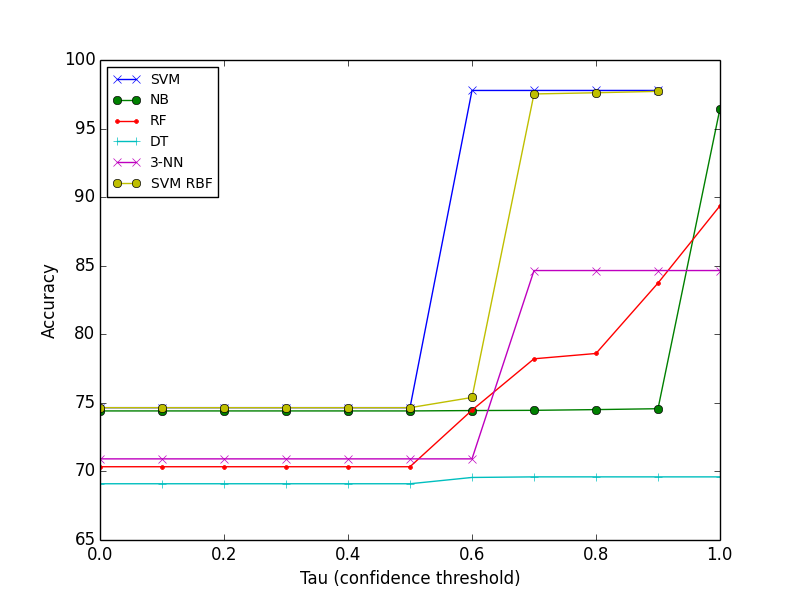
\includegraphics[width=3.1in]{../data/fig/tau-Accuracy}}
\subfigure[Phi]{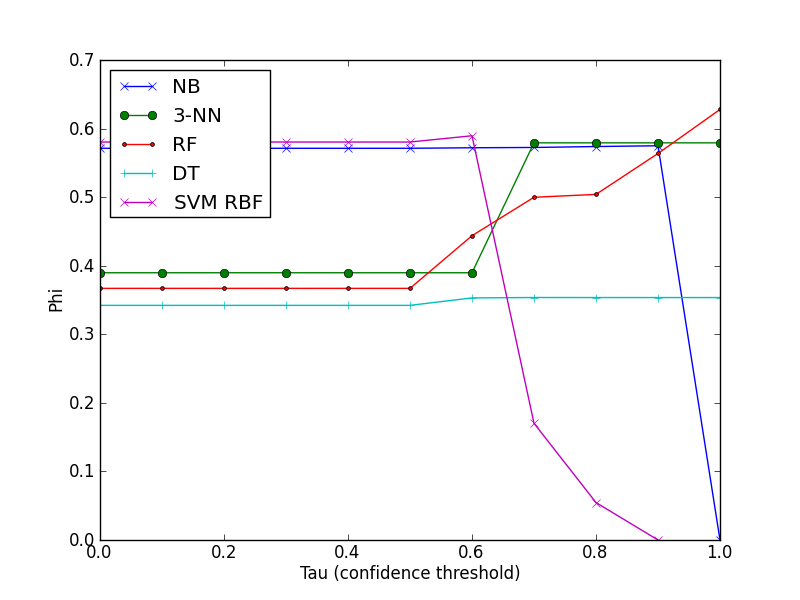
\includegraphics[width=3.1in]{../data/fig/tau-Phi}}
\subfigure[Recall]{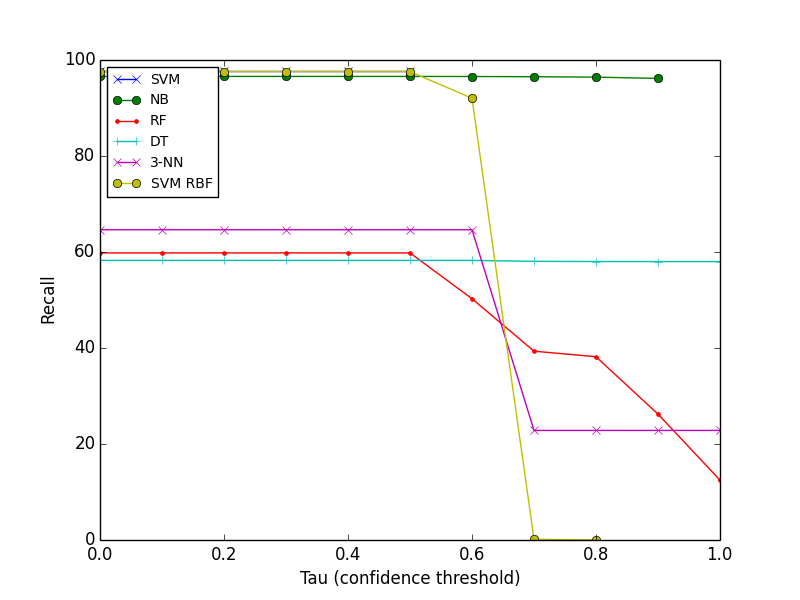
\includegraphics[width=3.1in]{../data/fig/tau-Recall}}
\subfigure[Precision]{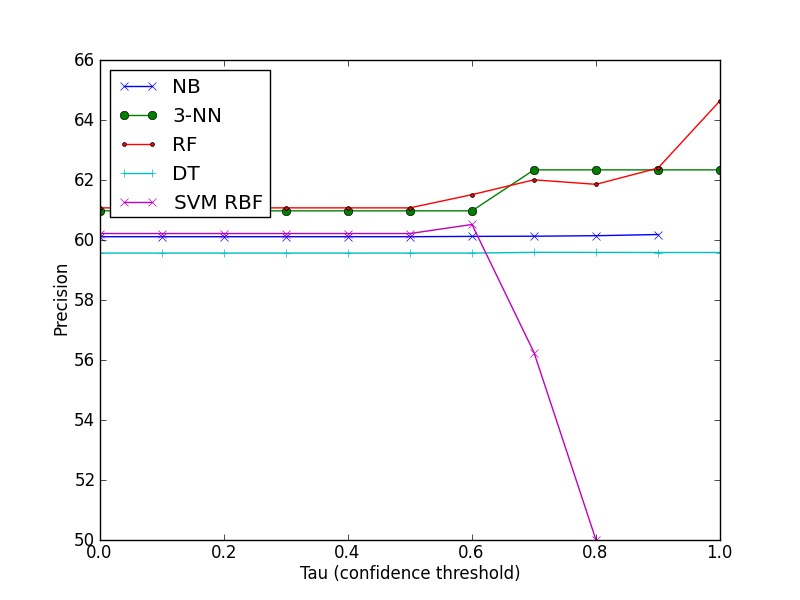
\includegraphics[width=3.1in]{../data/fig/tau-Precision}}
\subfigure[Efficiency]{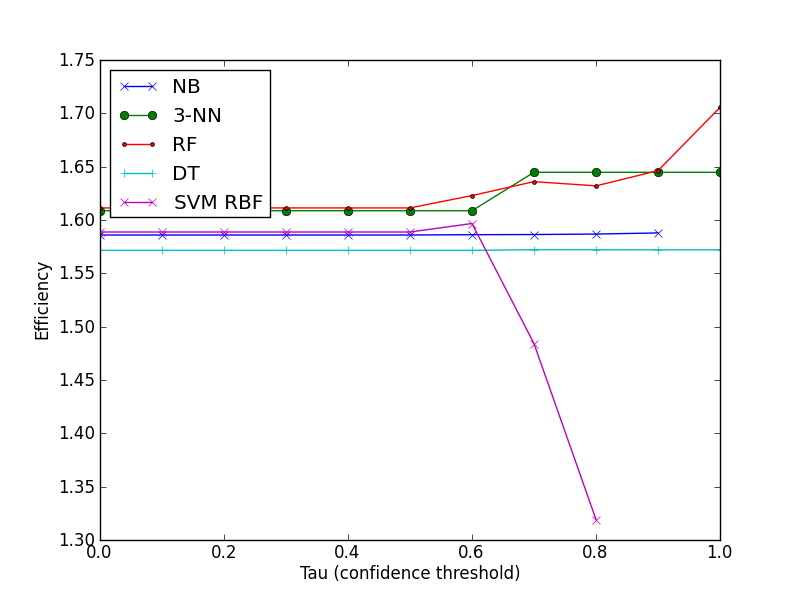
\includegraphics[width=3.1in]{../data/fig/tau-Efficiency}}
\caption{Classifier results in predicting weeding decisions when
  varying the confidence threshold, $\tau$.}
\label{fig:res}
\end{figure}


\section{Discussion of Results}

The level of agreement between machine and human weeding decisions
that was achieved using the current representation reached a maximum
of 0.57 (accuracy of 73.55\%), using a support vector machine.  While
this is statistically significant agreement, the large size of the
data set seems to render significant even low levels of agreement,
such as 0.16 (61.41\% accuracy) achieved by the 3-nearest-neighbor
classifier.  

All of the machine learning classifiers, except 3-nearest-neighbor,
performed better than either baseline approach in terms of accuracy.
This indicates that they successfully leveraged information in the
features.  However, they did not out-perform the ``Keep'' baseline by
a large margin.

\section{Next Steps}

Rather than relying on the machine to make predictions for all items,
we may observe higher agreement by retaining only the most confident
machine predictions.  Each classifier produces a confidence associated
with each prediction it makes.  We can use the machine output to rank
the items by decreasing confidence in a ``Withdraw'' outcome.  We will
assess accuracy and $\phi$ agreement for a number of different
confidence thresholds $t$, in which only items with predictions that
have confidence greater than $t$ will be considered.  This corresponds
to a realistic scenario in which a librarian might use the machine
predictions to prioritize candidates most likely to be weeded first.

Second, we will incorporate additional features into the item
representation:
\begin{itemize}
\item Item in Hathi trust (provided by Wesleyan)
\item Item in {\em Resources for College Libraries} (requires lookup by ISBN)
\end{itemize}



\end{document}
